\documentclass{beamer}
\usepackage{etoolbox}
\usepackage{tcolorbox}

\usetheme{Warsaw}

\title{Advanced Electrical}
\subtitle{UCB ME150A, Lecture 8}
\author[Ducky]{Ducky}
\date{March 19, 2014}

\makeatletter
\patchcmd{\beamer@sectionintoc}{\vskip1.5em}{\vskip0.5em}{}{}
\makeatother

\AtBeginSection[]
{
  \begin{frame}
    \frametitle{Table of Contents}
    \tableofcontents[currentsection,hideothersubsections]
  \end{frame}
}
\setbeamertemplate{sidebar right}{}
\setbeamertemplate{footline}{%
\hfill\usebeamertemplate***{navigation symbols}
\hspace{1cm}\insertframenumber{}/\inserttotalframenumber}

\begin{document}
% -------- -------- -------- -------- --------
\begin{frame}[plain] \centering
  \titlepage
  \begin{center} 
  \includegraphics[scale=0.5]{../images/external/ccbysa} \\
  \tiny This work is licensed under a Creative Commons \\
  Attribution-ShareAlike 3.0 International License \\
  ~ \\
  Source available on GitHub: \\
  \texttt{https://github.com/CalSol/training-docs/} \\
  ~ \\
  Photos from various Internet sources
   \end{center}
\end{frame}

\section{Common Circuits Blocks}
\begin{frame}{Introduction}
  \begin{itemize}
    \item Circuits are often made of modular sub-circuits, each providing some functionality
    \item Often, circuit blocks exist that are stock solutions to certain problems
    \begin{itemize}
      \item Like switching regulators for voltage regulation
      \item Or pull-up resistors for buttons
    \end{itemize}
    \item Using these prevents "reinventing the wheel" and makes circuits more readable, leveraging widespread familiarity
    \begin{itemize}
      \item Similar to patterns in software development
      \item Or mechanisms in mechanical engineering
    \end{itemize}
  \end{itemize}
  !!TODO:add circuit block pictures here
\end{frame}

\subsection{LED circuit}
\begin{frame}{LED circuit}
  \begin{columns}[T]
    \begin{column}{.6\textwidth}
	  LEDs are diodes that illuminate when current flows through them
      \begin{itemize}
        \item LEDs have maximum current ratings, so should not directly be connected to a voltage source
        \item Indicator LEDs typically consume ~20mA and drop 1-3V
        \item Use a resistor to limit current
        \item High power LEDs can consume much more current, and require specialized drive circuitry
      \end{itemize}
    \end{column}

    \begin{column}{0.4\textwidth} \centering
      \includegraphics[scale=0.5]{../images/circuit-blocks/led_vert_io} \\
      LED circuit \\
      ~ \\
      Use $R=\frac{V_s-V_f}{I_{LED}}$ \\
      {\tiny
        $V_s$ supply voltage \\
        $V_f$ LED voltage drop \\
        $I_{LED}$ LED current \\
      }
    \end{column}
  \end{columns}
\end{frame}

\subsection{Pull-up / pull-down}
\begin{frame}{Pull-up / pull-down networks}
  \begin{columns}[T]
    \begin{column}{.6\textwidth}
	  Pull-up / pull-down resistors connect a large resistor from a source (voltage supply or ground) to a line
      \begin{itemize}
        \item The resistor weakly pulls the line to the other side
        \item This provides a "default value" for the line, in the absence of other connections
        \item Pull-ups weakly connect a positive supply, while pull-downs weakly connect ground
      \end{itemize}
    \end{column}

    \begin{column}{0.4\textwidth} \centering
      \includegraphics[scale=0.5]{../images/circuit-blocks/pullup_vert_io} \\
      Pull-up circuit \\
      ~ \\
      \includegraphics[scale=0.5]{../images/circuit-blocks/pulldown_vert_io} \\
      Pull-down circuit
    \end{column}
  \end{columns}
\end{frame}

\begin{frame}{Floating lines and switches}
  \begin{columns}[T]
    \begin{column}{.6\textwidth}
	  Uses
      \begin{itemize}
        \item Prevent floating lines
        \begin{itemize}
          \item Disconnected lines "float" to indeterminiate voltages based on external noise - bad!
        \end{itemize}
        \item In switch circuits
        \begin{itemize}
          \item Where the switch "overpowers" the resistor when closed
          \item Can think of as a (lopsided) voltage divider when closed
          \item Convention: switches connected to ground, but weakly pulled up
        \end{itemize}
        \item Voltage shifting
        \begin{itemize}
          \item Replace switch with a transistor
        \end{itemize}
      \end{itemize}
    \end{column}

    \begin{column}{0.4\textwidth} \centering
      \includegraphics[scale=0.5]{../images/circuit-blocks/pullup_switch_open}
      \includegraphics[scale=0.5]{../images/circuit-blocks/pullup_switch_closed} \\
      Pull-up circuit with switch
    \end{column}
  \end{columns}
\end{frame}

\subsection{Op-amps}
\begin{frame}{Opamps}
  \begin{columns}[T]
    \begin{column}{.6\textwidth}
      \only<1>{
      \begin{itemize}
        \item Op-amps ("operational amplifiers") are amplifiers with very high gain
        \begin{itemize}
          \item ... which in itself, isn't very useful
        \end{itemize}
        \item Common connected in circuits with negative feedback for various applications:
        \begin{itemize}
          \item Buffer (1:1 input:output voltage)
          \item Inverting/noninverting amplifiers
        \end{itemize}
        \item Or with positive feedback:
        \begin{itemize}
          \item Schmitt trigger (comparartor with hysteresis)
          \item Oscillators
        \end{itemize}
      \end{itemize}
      }
      \only<2>{
      \begin{itemize}
        \item Op-amps are commonly used in analog circuits and for signal processing
        \item A detailed description is outside the scope of this lecture
        \begin{itemize}
          \item being a significant chunk of EE40, covering several lectures
        \end{itemize}
        \item But at least you know they exist, and what they can be used for
      \end{itemize}
      }
    \end{column}

    \begin{column}{0.4\textwidth} \centering
      \includegraphics[scale=0.5]{../images/symbols/opamp_labeled} \\
      \includegraphics[scale=0.5]{../images/circuit-blocks/opamp_noninvertingamp} \\
      Non-inverting amplifier \\
      $V_{out}=V_{in}(1+\frac{R_f}{R_g})$
    \end{column}
  \end{columns}
\end{frame}

\subsection{Power Systems}
\begin{frame}{Power Systems}
  \begin{columns}[T]
    \begin{column}{.6\textwidth}
      \begin{itemize}
        \item Circuits are useless without power
        \begin{itemize}
          \item Often need a battery or connector to a power brick
        \end{itemize}
        \item Most circuits need well-regulated DC power, providing stable voltage
        \begin{itemize}
          \item Bad quality power supplies may be instable as power load varies
          \item Battery voltage drops as depleted
          \item Some supplies are AC
        \end{itemize}        
      \end{itemize}
    \end{column}

    \begin{column}{0.4\textwidth} \centering
      \includegraphics[scale=0.5]{../images/symbols/sourcedc_labeled}
      \includegraphics[scale=0.5]{../images/symbols/sourceac_labeled} \\
      DC and AC voltage sources \\
      \includegraphics[scale=0.5]{../images/symbols/battery_labeled} \\
      Battery
    \end{column}
  \end{columns}
\end{frame}

\begin{frame}{Rectifiers}
  \begin{columns}[T]
    \begin{column}{.6\textwidth}
      \begin{itemize}
        \item Rectifiers convert AC to DC
        \item Diodes prevent reverse voltage
        \begin{itemize}
          \item Simple, but is only a half-wave rectifier (negative voltage suppressed)
          \item Incurs one diode voltage drop
        \end{itemize}
        \item Bridge rectifiers 
        \begin{itemize}
          \item Rectifies input positive and negative voltages
          \item But uses 4 diodes, and incurs two diode voltage drops
        \end{itemize}        
      \end{itemize}
    \end{column}

    \begin{column}{0.4\textwidth} \centering
      \only<1>{
      !!TODO: halfwave rectifier with waves
      }
      \only<2>{
      !!TODO: fullwave rectifier with waves
      }
    \end{column}
  \end{columns}
\end{frame}

\begin{frame}{Linear regulators}
  \begin{columns}[T]
    \begin{column}{.6\textwidth}
      \begin{itemize}
        \item Linear regulators use active feedback to maintain a constant voltage on the output
        \begin{itemize}
          \item Internally, it's a self-adjusting resistive divider
        \end{itemize}
        \item Intuitively, power from the "excess" voltage is burned as heat
        \begin{itemize}
          \item Which is quite inefficient...
          \item Can get quite hot when handling a lot of power!
        \end{itemize}        
        \item Often a single chip - simple to use
        \item Provides fairly stable output power
      \end{itemize}
    \end{column}

    \begin{column}{0.4\textwidth} \centering
      \includegraphics[scale=0.5]{../images/circuit-blocks/7805} \\
      Linear regulator circuit with LM7805\\
      ~ \\
      \includegraphics[scale=0.5]{../images/physical/7805_to220_labeled} \\
    \end{column}
  \end{columns}
\end{frame}

\begin{frame}{Switching regulators}
  \begin{columns}[T]
    \begin{column}{.6\textwidth}
      \begin{itemize}
        \item Switching regulators use storage elements (inductors, capacitors) to regulate output voltage
        \begin{itemize}
          \item Power is not intentionally burned
          \item But there are losses (as heat) from nonidealities (resistance)
        \end{itemize}
        \item Buck converters step down an input voltage using inductors
        \item Boost converters step up an input voltage using inductors
        \item Switched-capacitor regulators use a flying capacitor
      \end{itemize}
    \end{column}

    \begin{column}{0.4\textwidth}
      !!TODO: Buck, boost circuits
    \end{column}
  \end{columns}
\end{frame}

\begin{frame}{Theory example: boost converters}
  \begin{columns}[T]
    \begin{column}{.6\textwidth}
      \begin{itemize}
        \item {\em Background}: Inductors
        \begin{itemize}
          \item Resist changes in current by adjusting voltage
        \end{itemize}
        \item When switch is closed:
        \begin{itemize}
          \item Inductor charges from the supply, increasing current through it
          \item Diode prevents backflow
        \end{itemize}
        \item When switch is open:
        \begin{itemize}
          \item Only path for inductor current is through the diode
          \item Inductor voltage increases to maintain constant current flow
        \end{itemize}
        \item Output voltage depends on switching duty cycle
      \end{itemize}
    \end{column}

    \begin{column}{0.4\textwidth}
      !!TODO: Boost diagram
    \end{column}
  \end{columns}
\end{frame}

\begin{frame}{Practical regulators}
  \begin{columns}[T]
    \begin{column}{.6\textwidth}
      \begin{itemize}
        \item Most regulators supplied as chips
        \item Adjustable-output versions available
        \begin{itemize}
          \item Regulate to keep feedback pin at constant voltage
          \item Use voltage divider from output to specify setpoint
          \item Internally, it's black magic (or EE120, take your pick)
        \end{itemize}
        \item Switching regulators have varyign degrees of integration
        \begin{itemize}
          \item Switch may be internal
          \item Or even internal chip-scale inductor
        \end{itemize}
      \end{itemize}
    \end{column}

    \begin{column}{0.4\textwidth}
      !!TODO: Toy boost regulator IC with integrated switch and adjustabout output
    \end{column}
  \end{columns}
\end{frame}

\subsection{Various ICs}
\begin{frame}{ICs: Integrated Circuits}
  \begin{columns}[T]
    \begin{column}{.6\textwidth}
      \begin{itemize}
        \item All kinds of specialized devices are available as integrated circuits:
        \item Logic
        \begin{itemize}
          \item Logic gates and level shifters
        \end{itemize}
        \item Sensors
        \begin{itemize}
          \item Illuminance sensors
          \item Temperature sensors
          \item Accelerometers, gyroscopes
        \end{itemize}
        \item Radio-frequency transceivers
        \item ASICs
        \begin{itemize}
          \item Bitcoin miners that never ship ...
        \end{itemize}
        \item And many, many more
      \end{itemize}
    \end{column}

    \begin{column}{0.4\textwidth} \centering
      \includegraphics[width=0.9\columnwidth]{../images/external/dogecoin_reddit_frame_wp0UDqp} \\
      Yes, there are dedicated chips for this
    \end{column}
  \end{columns}
\end{frame}

\section{Electrical Design Principles}
\begin{frame}{Introduction}
  \begin{columns}[T]
    \begin{column}{.6\textwidth}
      \begin{itemize}
        \item Good design practices help prevent common mistakes
        \item Learn from others' failures, so you don't need to repeat them!
      \end{itemize}
    \end{column}

    \begin{column}{0.4\textwidth} \centering
      \includegraphics[width=0.9\columnwidth]{../images/external/laptopfire_engadget_dell-laptop-fire-new-1} \\
      "oops!"
    \end{column}
  \end{columns}
\end{frame}

\subsection{Understanding circuits}
\begin{frame}{Understanding circuits}
  \begin{columns}[T]
    \begin{column}{.6\textwidth}
      \begin{itemize}
        \item Designing circuits often involves copying and modifying a supplied reference circuit
        \item Make sure you understand it!
        \begin{itemize}
          \item (within reason, of course)
          \item Otherwise, you may make lulzworthy mistakes...
        \end{itemize}
      \end{itemize}
      \begin{tcolorbox}[] \centering
      \underline{if you remember nothing else:} \\
      ALWAYS UNDERSTAND WHAT YOU'RE DESIGNING!
      \end{tcolorbox}
    \end{column}

    \begin{column}{0.4\textwidth} \centering
      \includegraphics[scale=0.25]{../images/external/hangman_thisbluemarble} \\
      Don't let this happen to you!
    \end{column}
  \end{columns}
\end{frame}

\subsection{Maximum ratings}
\begin{frame}{Maximum ratings}
  \begin{columns}[T]
    \begin{column}{.6\textwidth}
      \begin{itemize}
        \item Most components have maximum ratings: follow them!
        \item Maximum voltage/current ratings
        \item Operating/storage temperatures
        \begin{itemize}
          \item before permanent damage, either obvious or latent
        \end{itemize}
        \item Maximum frequency ratings
        \begin{itemize}
          \item before outputs are incorrect
        \end{itemize}
        \item Parts must {\em always} be within spec
        \begin{itemize}
          \item consider boundary conditions, like circuit start-up and shut-down
        \end{itemize}
      \end{itemize}
    \end{column}

    \begin{column}{0.4\textwidth} \centering
      \includegraphics[scale=0.2]{../images/external/LM7805_absolutemaxratings} \\
      Absolute maximum ratings for LM7805
    \end{column}
  \end{columns}
\end{frame}

\subsection{Robust design}
\begin{frame}{Idiot-proofing}
  \begin{columns}[T]
    \begin{column}{.6\textwidth}
      \begin{itemize}
        \item Idiot-proofing is general good engineering practice
        \begin{itemize}
          \item Not because we're idiots
          \item But not everone's had their morning coffee
          \item Or more relevantly, sleep
        \end{itemize}
        \item Electrical idiot-proofing
        \begin{itemize}
          \item Different connectors
          \item Polarized connectors, preventing reversed insertion
          \item Labeling boards for debugging
        \end{itemize}
      \end{itemize}
    \end{column}

    \begin{column}{0.4\textwidth} \centering
      \includegraphics[width=0.9\columnwidth]{../images/external/tritium_calsol} \\
      "they just make better idiots" \\
      {\tiny A CalSol true story}
    \end{column}
  \end{columns}
\end{frame}

\begin{frame}{Protection}
  \begin{columns}[T]
    \begin{column}{.6\textwidth}
      \begin{itemize}
        \item Prevent malfunctions from becoming catastrophies
        \item Fuses / circuit breakers
        \begin{itemize}
          \item Prevent excessive overcurrent by breaking the circuit
        \end{itemize}
        \item Self-resetting fuses
        \begin{itemize}
          \item Use temperature rise from overcurrent to (nonlinearly) increase resistance
          \item As current drops, temperature decreases and fuse "resets"
          \item Good to have on power inputs
        \end{itemize}
      \end{itemize}
    \end{column}

    \begin{column}{0.4\textwidth} \centering
      \includegraphics[width=0.9\columnwidth]{../images/external/polyfuse_wikipedia_publicdomain_800px-Photo-Polyswitch} \\
      Self-resetting fuses \\
    \end{column}
  \end{columns}
\end{frame}

\begin{frame}{Protection}
  \begin{columns}[T]
    \begin{column}{.6\textwidth}
      \begin{itemize}
        \item Minimize damage from misuse
        \item ESD / TVS Suppression
        \begin{itemize}
          \item ESD: Electrostatic Discharge, typically on order of kilovolts (enough to destroy modern ICs)
          \item Causes: static accumulates on people and machines
          \item Fast-acting diodes dump excess voltage to ground
          \item Good to have on connectors
        \end{itemize}
      \end{itemize}
    \end{column}

    \begin{column}{0.4\textwidth}
      !!TODO: protection circuits: ESD diodes, warning
    \end{column}
  \end{columns}
\end{frame}

\subsection{Standardization}
\begin{frame}{Standardization}
  \begin{columns}[T]
    \begin{column}{.6\textwidth}
      \begin{itemize}
        \item Use standard parts
        \begin{itemize}
          \item Reduce inventory overhead
          \item Buy in bulk
        \end{itemize}
        \item Common packages for components
        \begin{itemize}
          \item Through-hole: various axial sizes (1/4 watt, ...)
          \item Surface-mount: various sizes (0402, 0603, 0805, ...)
        \end{itemize}
        \item Common values for components
        \begin{itemize}
          \item E series of preferred numbers
          \item E6 series: 10, 15, 22, 33, 47, 68
        \end{itemize}
      \end{itemize}
    \end{column}

    \begin{column}{0.4\textwidth} \centering
      \includegraphics[width=0.9\columnwidth]{../images/external/smd_wikipedia_publicdomain_Photo-SMDcapacitors} \\
      Various components in various standardized sizes
    \end{column}
  \end{columns}
\end{frame}

\subsection{Design for Test}
% to be written

\section{PCB Design}
\begin{frame}{Introduction: circuit technologies}
  \begin{columns}[T]
    \begin{column}{.6\textwidth}
      Common ways to realize circuits:
      \begin{itemize}
        \item Breadboard
        \begin{itemize}
          \item For early prototyping
          \item Literally, plug and play
          \item Not stable or for production use
        \end{itemize}
        \item Protoboard
        \begin{itemize}
          \item Parts soldered onto grid of holes - more permanent than breadboard
          \item Time consuming to assemble
          \item Not suitable for small, surface-mount parts
        \end{itemize}
      \end{itemize}
    \end{column}

    \begin{column}{0.4\textwidth} \centering
      \includegraphics[width=0.9\columnwidth]{../images/external/breadboarclear_mouser_BPS-IMG-BB400T} \\
      \includegraphics[scale=0.15]{../images/breadboard/internals} \\
      Breadboard and internal connections
    \end{column}
  \end{columns}
\end{frame}

\subsection{PCB overview}
\begin{frame}{PCBs}
  \begin{columns}[T]
    \begin{column}{.6\textwidth}
      PCB: Printed Circuit Board
      \begin{itemize}
        \item Is a substrate (typically fiberglass, FR-4) with layers of copper etched into tracks and pads
        \begin{itemize}
          \item Most have top and bottom copper layers, to which parts can be attached
          \item Complicated designs have internal copper layers
          \item Plated holes (vias) connect layers
          \item Silkscreen for labels and art
        \end{itemize}
        \item Used for mass-production
        \item So, how do we design one?
      \end{itemize}
    \end{column}

    \begin{column}{0.4\textwidth} \centering
      \includegraphics[scale=0.5]{../images/pcb/stackup} \\
      PCB stackup
    \end{column}
  \end{columns}
\end{frame}

\subsection{Schematic capture}
\begin{frame}{Schematic Capture}
  \begin{columns}[T]
    \begin{column}{.6\textwidth}
      Schematic capture
      \begin{itemize}
        \item Is entering a circuit schematic into the computer
        \begin{itemize}
          \item Manipulate symbols (abstract representations of components) around a schematic
          \item Connect pins to make a circuit
          \item Modern tools {\em typically} intuitive
        \end{itemize}
        \item is NOT a physical layout
        \begin{itemize}
          \item Design for readability: create modular and neat schematics
          \item Can have implicit wires, like voltage rails and tunnels
        \end{itemize}
      \end{itemize}
    \end{column}

    \begin{column}{0.4\textwidth} \centering
      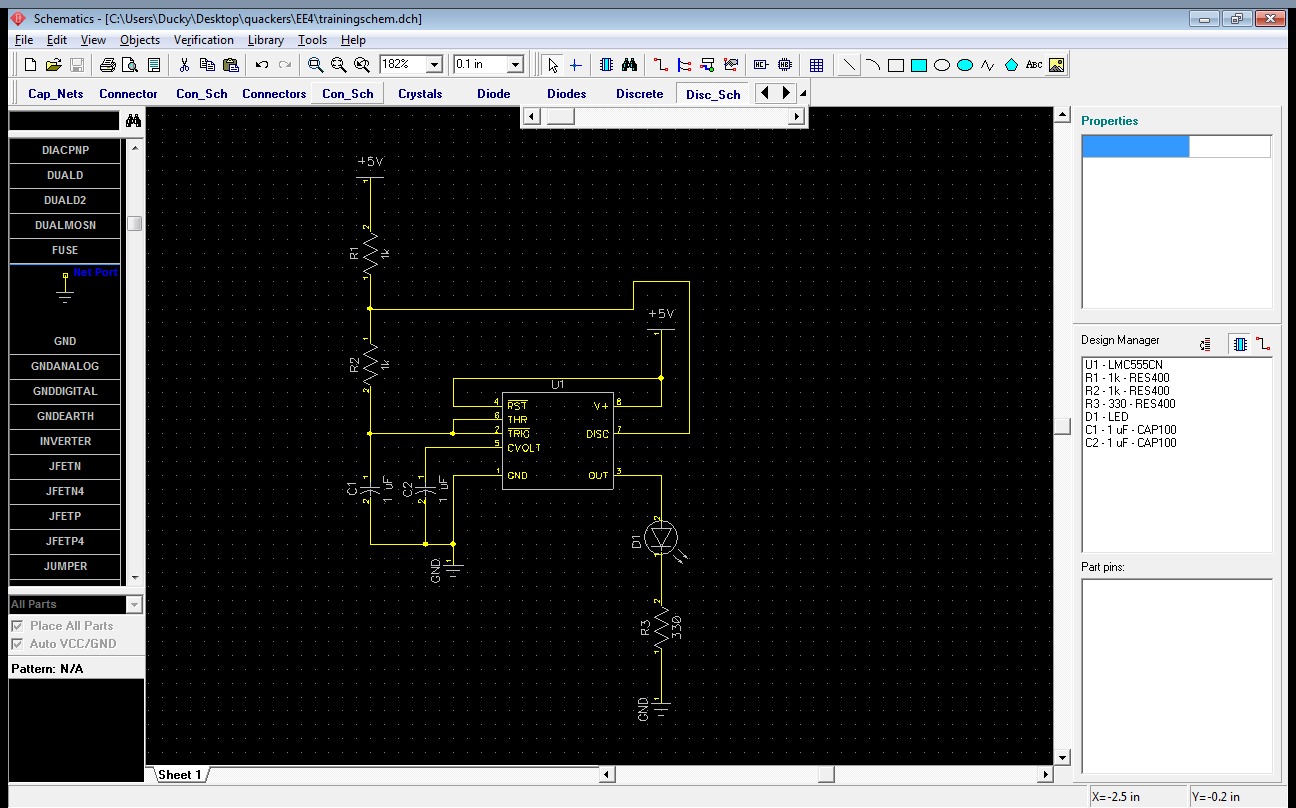
\includegraphics[width=0.9\columnwidth]{../images/diptrace/555_schematic} \\
      Schematic capture tool
    \end{column}
  \end{columns}
\end{frame}

\subsection{Board layout}
\begin{frame}{Board layout}
  \begin{columns}[T]
    \begin{column}{.6\textwidth}
      Board layout
      \begin{itemize}
        \item Is doing the physical layout
        \begin{itemize}
          \item Tools automatically convert schematic representation to physical representation
          \item Position component footprints
          \item Then route traces (wires) between pins
        \end{itemize}
        \item Footprints are the board "artwork" for each component
        \begin{itemize}
          \item Including copper pads/holes which component leads/pins are soldered to
          \item and silkscreen labels/outlines
        \end{itemize}
      \end{itemize}
    \end{column}

    \begin{column}{0.4\textwidth} \centering
      \includegraphics[scale=0.5]{../images/physical/555_dip8_labeled} \\
      \includegraphics[scale=0.4]{../images/physical/footprint_dip8}
      \includegraphics[scale=0.4]{../images/physical/footprint_dip8_populated} \\
      Chip, footprint, and board
    \end{column}
  \end{columns}
\end{frame}

\begin{frame}{Constraints}
  \begin{columns}[T]
    \begin{column}{.6\textwidth}
      \begin{itemize}
        \item Have to meet design rules, dictated by fab capability:
        \begin{itemize}
          \item Minimum trace width/spacing
          \item Minimum/maximum hole size
          \item ... and more
          \item Tools can check for these
        \end{itemize}
        \item ... along with other constraints:
        \begin{itemize}
          \item Signal integrity, especially for high-speed signals
          \item Trace resistances
          \item interference
        \end{itemize}
      \end{itemize}
    \end{column}

    \begin{column}{0.4\textwidth} \centering
      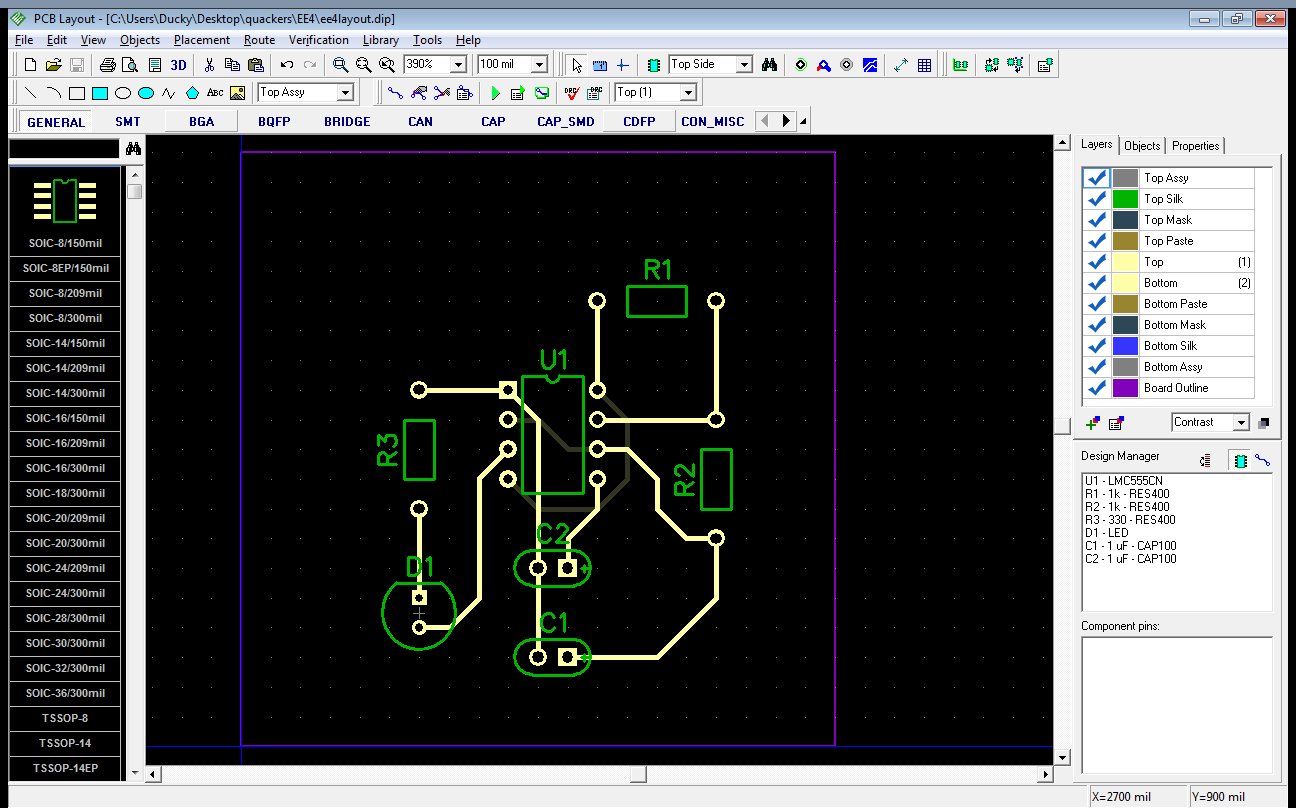
\includegraphics[width=0.9\columnwidth]{../images/diptrace/555_layout} \\
      Board layout tool
    \end{column}
  \end{columns}
\end{frame}

\begin{frame}{Good practices}
  \begin{columns}[T]
    \begin{column}{.6\textwidth}
      \begin{itemize}
        \item Good layout practices:
        \begin{itemize}
          \item Plan ahead: placement determines routing difficulty
          \item Don't design for minimums unless necessary
          \item Avoid overlapping components
          \item Ensure board is easy to assemble
        \end{itemize}
        \item Generally, part science, {\em part art}:
        \begin{itemize}
          \item Align parts to a grid
          \item Use patterns where appropriate
          \item Conventionally, traces routed at 45 degree angles
          \item Make it pretty!
        \end{itemize}
      \end{itemize}
    \end{column}

    \begin{column}{0.4\textwidth} \centering
      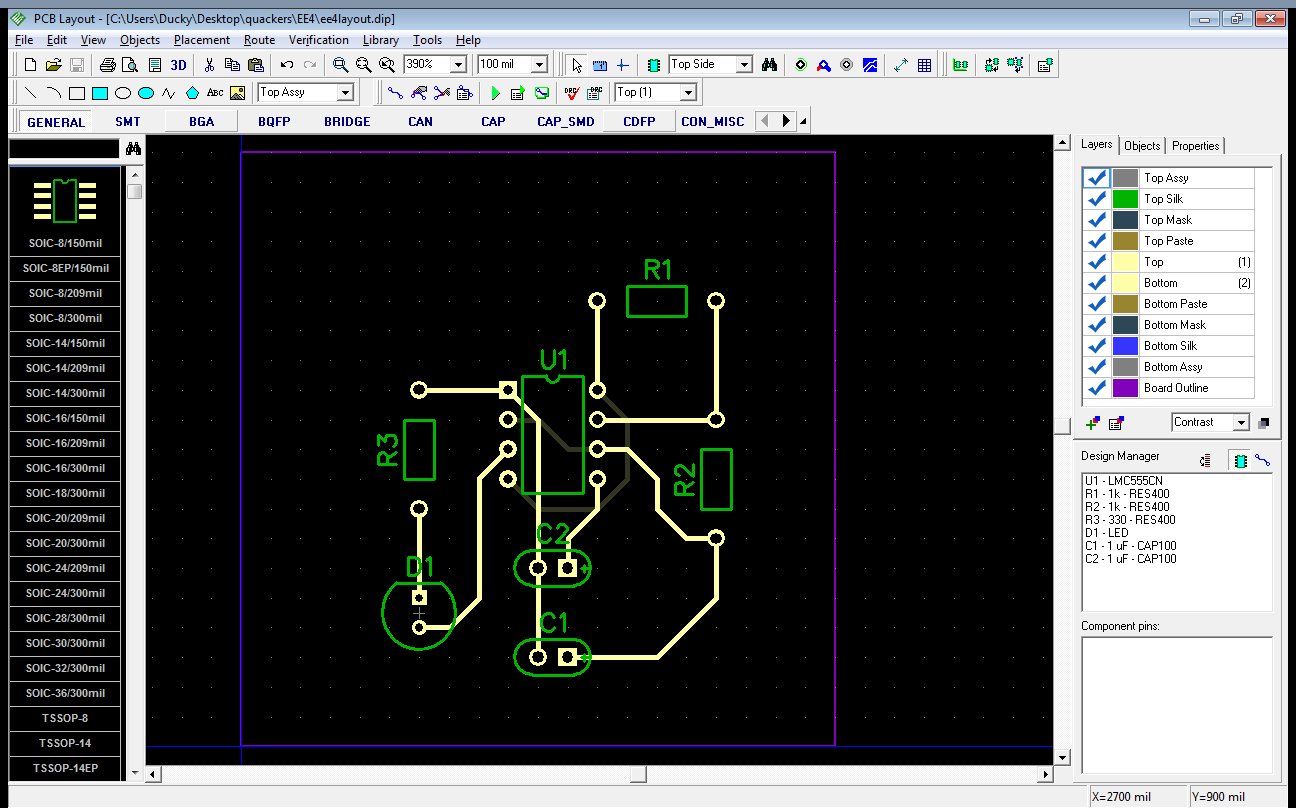
\includegraphics[width=0.9\columnwidth]{../images/diptrace/555_layout} \\
      Board layout tool
      %TODO: more descriptive image here
    \end{column}
  \end{columns}
\end{frame}

\subsection{Fabrication}
\begin{frame}{Fabrication}
  \begin{columns}[T]
    \begin{column}{.6\textwidth}
      \begin{itemize}
        \item Tools export board design as Gerber files (RS-274X)
        \begin{itemize}
          \item ... no, not the baby food ...
          \item RS-274X is a standard for artwork for board layers (board shape, copper, silkscreen, ...)
          \item Uniersally accepted by board fabrication houses
        \end{itemize}
      \end{itemize}
    \end{column}

    \begin{column}{0.4\textwidth} \centering
      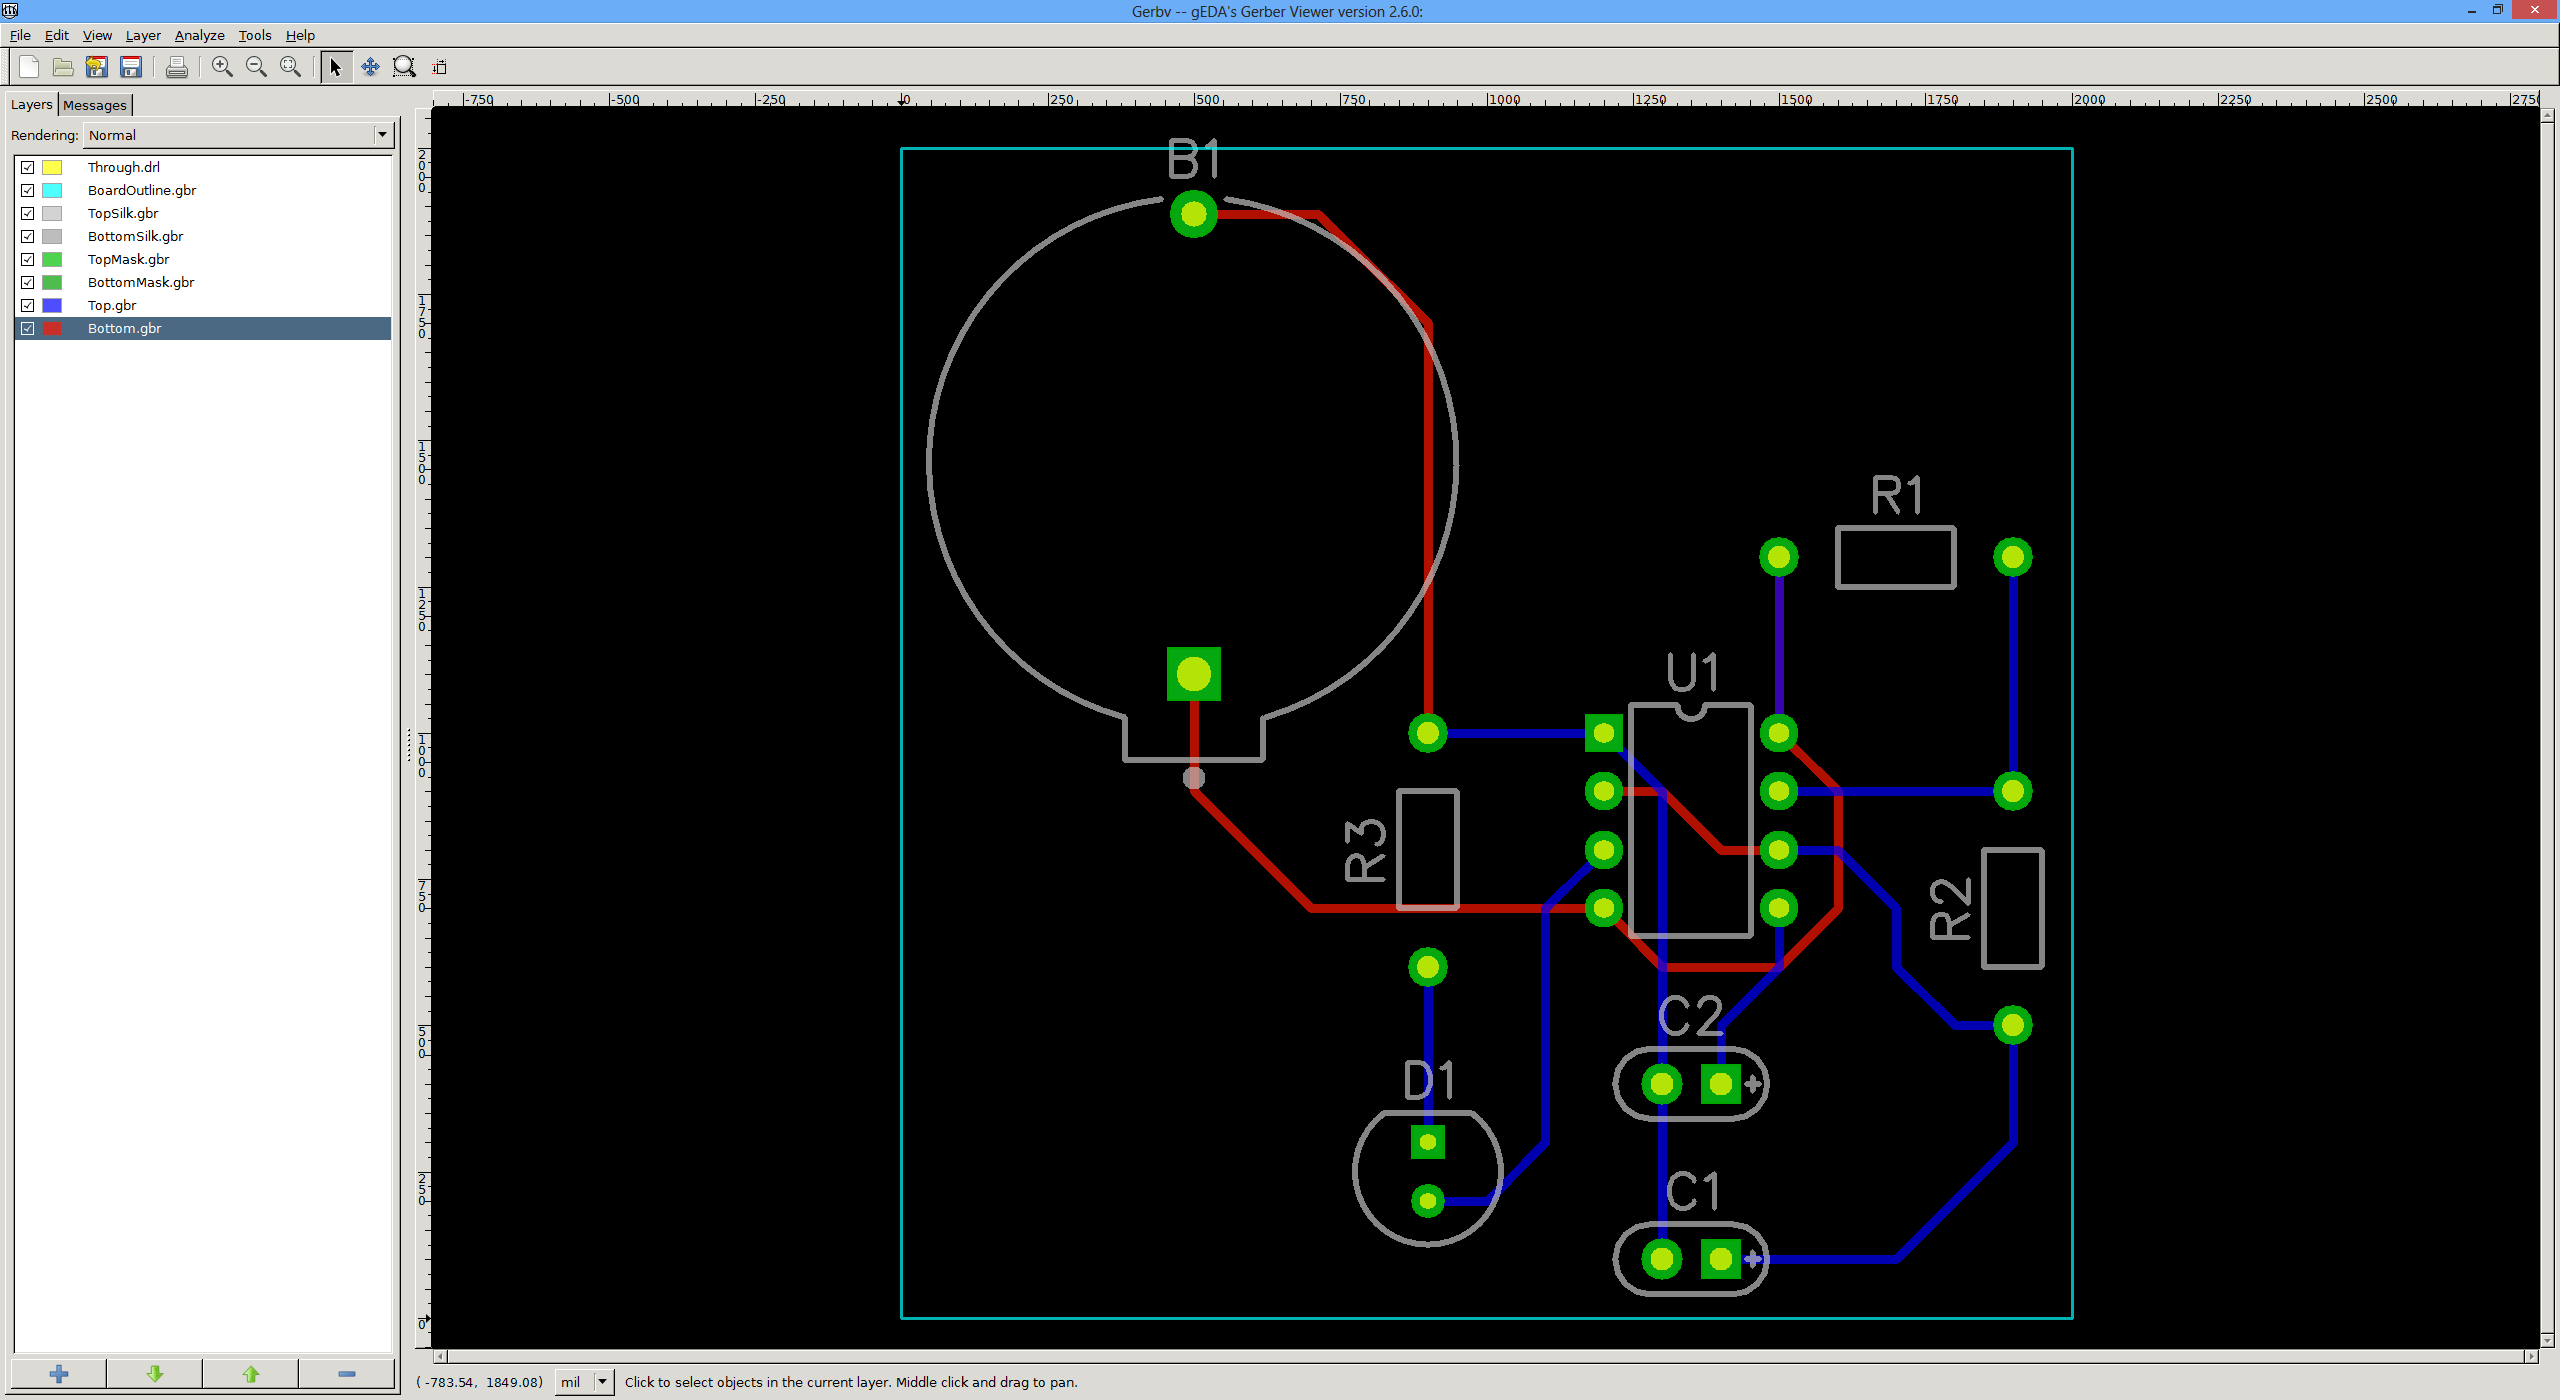
\includegraphics[width=0.9\columnwidth]{../images/diptrace/555_gerbv} \\
      Gerber files
    \end{column}
  \end{columns}
\end{frame}

\begin{frame}{Fabrication}
  \begin{columns}[T]
    \begin{column}{.6\textwidth}
      \begin{itemize}
        \item Send design files to board house, pay costs, and wait
        \begin{itemize}
          \item Prototyping costs (small runs): typically \$2.50 - \$5.00 per sq.in for two copper layers
          \item Mass production costs: cheap!
          \item Most of fab cost is start-up costs, per-design rather than per-board
        \end{itemize}
        \item Boards mailed in about a week
      \end{itemize}
    \end{column}

    \begin{column}{0.4\textwidth}
      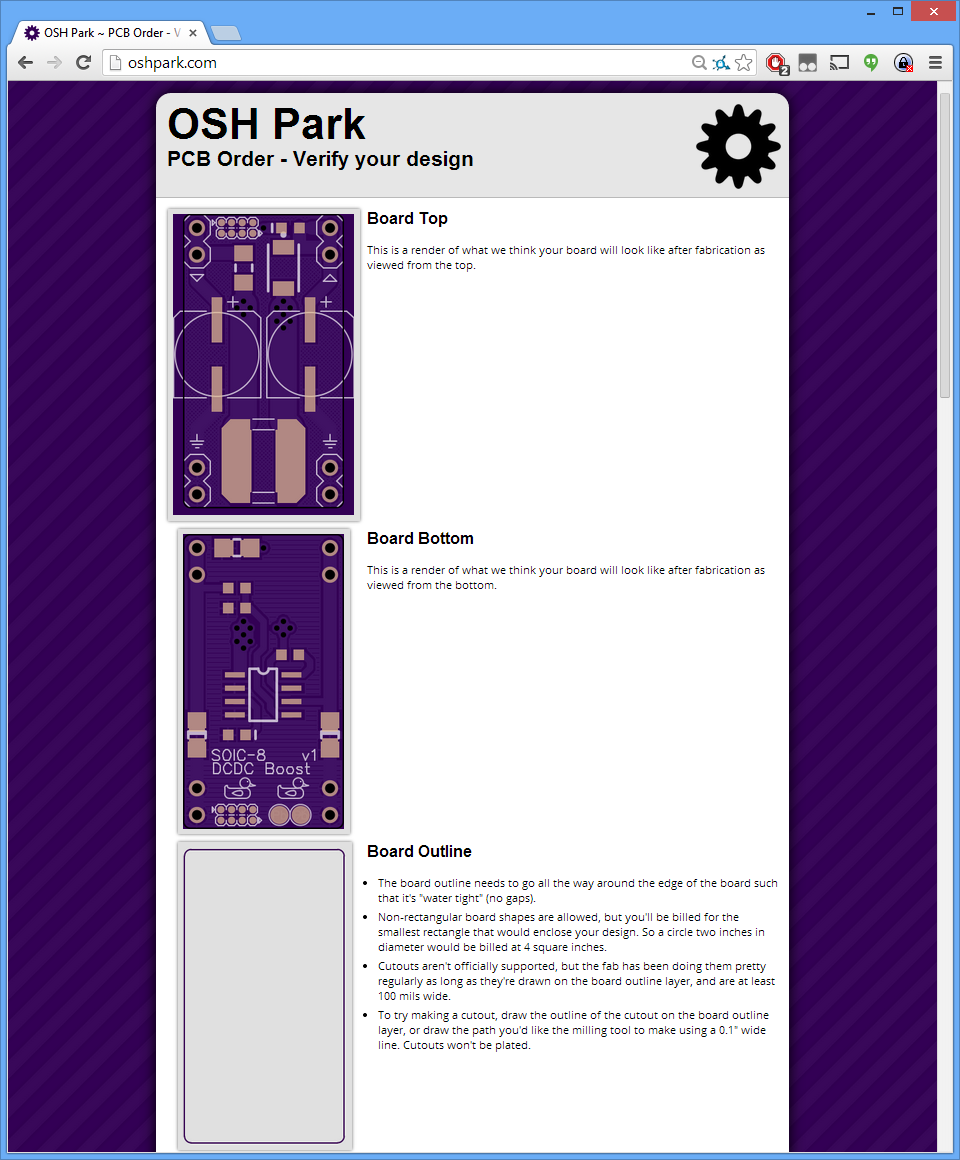
\includegraphics[width=0.9\columnwidth]{../images/diptrace/dcdc_oshpark} \\
      Design being submitted at OSHPark
    \end{column}
  \end{columns}
\end{frame}

\subsection{}
\begin{frame}{Live demo (time permitting)}
\end{frame}

\begin{frame}[plain]
\frametitle{Break!} \centering
  Ask questions, or just sit back and chillax! \\
  ~ \\
  ~ \\
  \includegraphics[width=0.75\columnwidth]{../images/external/snorlax_bulbapedia_143Snorlax_OS_anime_2} 
\end{frame}

\section{Microcontrollers}
\begin{frame}{Introduction}
  \begin{columns}[T]
    \begin{column}{.6\textwidth}
      Microcontrollers
      \begin{itemize}
        \item Are chips with a processor core, memory, and input/output peripherals
        \begin{itemize}
          \item Essentially a complete (but simple) computer on a chip
        \end{itemize}
        \item Allows control of an electrical physical system from software
        \begin{itemize}
          \item Usually easier to reason about than circuit components
        \end{itemize}        
      \end{itemize}
    \end{column}

    \begin{column}{0.4\textwidth} \centering
      \includegraphics[width=.9\columnwidth]{../images/external/mcu_wikipedia_publicdomain_PIC18F8720} \\
      An entire computer on a chip
    \end{column}
  \end{columns}
\end{frame}

\subsection{IOs and peripherals}
\begin{frame}{Overview}
  \begin{columns}[T]
    \begin{column}{.6\textwidth}
      IOs and peripherals
      \begin{itemize}
        \item Are how microcontrollers interact with the world around them
        \begin{itemize}
          \item Pins assert and detect electrical signals, which can be controlled from within hardware
        \end{itemize}
        \item Digital peripherals
        \begin{itemize}
          \item with with digital quantities, generally 0 and 1 (represented as high and low voltages)
        \end{itemize}
        \item Analog peripherals
        \begin{itemize}
          \item work with continuous quantities, but are usually quantized
        \end{itemize}
      \end{itemize}
    \end{column}

    \begin{column}{0.4\textwidth} \centering
      \includegraphics[width=.9\columnwidth]{../images/external/mcublockdiagram_microchip_pic18f_39609b} \\
      Microcontroller block diagram
    \end{column}
  \end{columns}
\end{frame}

\begin{frame}{Digital GPIO}
  \begin{columns}[T]
    \begin{column}{.6\textwidth}
      GPIO: General Purpose Input/Output
      \begin{itemize}
        \item Can be configuired as a digital input or output
        \item As an input:
        \begin{itemize}
          \item Can read the pin level
          \item Some chips have optional integrated pull-ups/pull-downs
          \item Example: read switch
        \end{itemize}
        \item As an output:
        \begin{itemize}
          \item Can assert a voltage (chip positive or negative supply)
          \item Example: drive LED
        \end{itemize}
      \end{itemize}
    \end{column}

    \begin{column}{0.4\textwidth} \centering
      \includegraphics[scale=0.5]{../images/circuit-blocks/led_vert_mcu}
      \includegraphics[scale=0.5]{../images/circuit-blocks/pullup_switch_mcu} \\
      Example LED and switch circuits through GPIO
    \end{column}
  \end{columns}
\end{frame}

\begin{frame}{Digital Communications}
  \begin{columns}[T]
    \begin{column}{.6\textwidth}
      Various digital signaling standards
      \begin{itemize}
        \item Parallel protocols:
        \begin{itemize}
          \item One line for each bit in word
          \item (entire word shifted out at once)
        \end{itemize}
        \item Serial protocols:
        \begin{itemize}
          \item Bits in a word shifted out one after the other
          \item (in a time-varying signal)
        \end{itemize}
        \item Example:
        \begin{itemize}
          \item UART (serial; two wires) often used for text console
          \item SPI (serial, 3 wires + select), I2C (serial; 2 wires) often used for inter-chip communication
        \end{itemize}
      \end{itemize}
    \end{column}

    \begin{column}{0.4\textwidth} \centering
      \includegraphics[scale=0.33]{../images/circuit-blocks/uart} \\
      Example UART hookup \\
      ~ \\
      \includegraphics[scale=0.25]{../images/circuit-blocks/i2c} \\
      Example I2C hookup
    \end{column}
  \end{columns}
\end{frame}

\begin{frame}{Analog Peripherals}
  \begin{columns}[T]
    \begin{column}{.6\textwidth}
      ADC (Analog to Digital converter)
      \begin{itemize}
        \item Reads a voltage level on a pin, and quantizes it to a digital value
        \begin{itemize}
          \item Resolution specified in bits
          \item Useful for sensing applications
        \end{itemize}
      \end{itemize}
      \phantom{x}
      DAC (Digital to Analog converter)
      \begin{itemize}
        \item Sets a voltage level on a pin
        \begin{itemize}
          \item Controlled from software
        \end{itemize}
      \end{itemize}
    \end{column}

    \begin{column}{0.4\textwidth} \centering
      \includegraphics[scale=0.5]{../images/circuit-blocks/pot_mcu} \\
      Example ADC circuit reading from potentiometer
    \end{column}
  \end{columns}
\end{frame}

\section{Programming}
\subsection{The C language}
\begin{frame}{The C language}
  \begin{columns}[T]
    \begin{column}{.6\textwidth}
      Most microcontrollers programmed in the C-language, which is:
      \begin{itemize}
        \item Imperative: statements executed in program order
        \item Procedural: code can be put into functions, which can be called
        \item Structured: block control structures
      \end{itemize}
      (no, you don't need to memorize this, but it helps to know the big ideas)
    \end{column}

    \begin{column}{0.4\textwidth}
      !!TODO: example code
    \end{column}
  \end{columns}
\end{frame}

\begin{frame}{C variables and functions}
  \begin{columns}[T]
    \begin{column}{.6\textwidth}
      Variables:
      \begin{itemize}
        \item Hold some type of data
        \item In C, have to be defined before use
        \item Can be assigned a new value
      \end{itemize}
      Functions:
      \begin{itemize}
        \item Have a signature: the types they take in (arguments) and return
        \item Contain some code, which may modify global state
        \item Can be called from other code
      \end{itemize}
    \end{column}

    \begin{column}{0.4\textwidth}
      !!TODO: example code, variable definition and functions
    \end{column}
  \end{columns}
\end{frame}

\begin{frame}{C conditional structures}
  \begin{columns}[T]
    \begin{column}{.6\textwidth}
      If:
      \begin{itemize}
        \item If executes code in a block if the condition evaluates true
        \item Can also have 'else if' block to test additional conditions if the previous are false
        \item And an 'else' block should none of the previous be true
      \end{itemize}
    \end{column}

    \begin{column}{0.4\textwidth}
      !!TODO: example code, if block else if
    \end{column}
  \end{columns}
\end{frame}

\begin{frame}{C loop structures}
  \begin{columns}[T]
    \begin{column}{.6\textwidth}
      Loops:
      \begin{itemize}
        \item Various loop constructs exist which executes code blocks multiple times
      \end{itemize}  
      For loops:
      \begin{itemize}
        \item Possibly the most common loop
        \item Contains:
        \begin{itemize}
          \item Initializer: executed once at start
          \item Condition: loop repeats if true
          \item Increment: executed at end of each loop
        \end{itemize}
      \end{itemize}
      Do-while loops:      
      \begin{itemize}
        \item Repeats as long as condition true
      \end{itemize}
    \end{column}

    \begin{column}{0.4\textwidth}
      !!TODO: example code, for loop
    \end{column}
  \end{columns}
\end{frame}

% TODO: add a section on running time and memory constraints, maybe

\subsection{Peripheral}
\begin{frame}{Using peripherals: functional abstraction}
  \begin{columns}[T]
    \begin{column}{.6\textwidth}
      \begin{itemize}
        \item Code to interact with microcontroller peripherals is usually supplied by the chip vendor as a library
        \begin{itemize}
          \item Documentation (of varying quality) is also provided, describing usage
        \end{itemize}
        \item Code is supplied as functions that perform some action when called:
        \begin{itemize}
          \item Set a GPIO output
          \item Return a quantized ADC value
          \item Shift a word out of a digital communications peripheral
        \end{itemize}        
      \end{itemize}
    \end{column}

    \begin{column}{0.4\textwidth}
      !!TODO: example GPIO code
    \end{column}
  \end{columns}
\end{frame}

\begin{frame}{Polling}
  \begin{columns}[T]
    \begin{column}{.6\textwidth}
      Often, need to react to events \newline
      \newline
      Polling:
      \begin{itemize}
        \item Repeatedly checks if condition true
        \item Do something if true, nothing if not
        \item Pros: simple to write
        \item Cons: wasted processing time repeatedly checking for condition (high overhead)
      \end{itemize}
    \end{column}

    \begin{column}{0.4\textwidth}
      !!TODO: example polling code to wait for switch
    \end{column}
  \end{columns}
\end{frame}

\begin{frame}{Asynchronous IO}
  \begin{columns}[T]
    \begin{column}{.6\textwidth}
      Asynchronous IO:
      \begin{itemize}
        \item Instead of repeatedly checking, notify on event
        \item Interrupt: jump to code block on event, needs hardware support
        \begin{itemize}
          \item Typical mechanism for hardware events on microcontrollers
          \item But tricky to get right
        \end{itemize}
        \item Callback: call a specified function when an event happens
        \begin{itemize}
          \item Typically a wrapper around an interrupt for microcontrollers
        \end{itemize}
      \end{itemize}
    \end{column}

    \begin{column}{0.4\textwidth}
      !!TODO: example async code to wait for switch
    \end{column}
  \end{columns}
\end{frame}

\subsection{}
\begin{frame}{Live demo (time permitting)}
\end{frame}

\begin{frame}[plain]
\frametitle{The end!} \centering
  Questions? \\
  ~ \\
  ~ \\
  \includegraphics[width=.75\columnwidth]{../images/external/800px-Ducks_Yerevan}
\end{frame}

\end{document}
